% First of all, include a document class and options
\documentclass[english,bachelor]{diploma}
% There are some addtional packages
\usepackage[autostyle=true]{csquotes} % enhanced support for quotation marks, support for biblatex package
\usepackage[backend=biber, style=iso-numeric, alldates=iso]{biblatex} % bibliography
\usepackage{dcolumn} % numeric column type
\usepackage{subfig} % subtables and subfigures
\usepackage[cpp]{diplomalst}

% Next, enter data for leading pages
\ThesisAuthor{Jonáš Koziorek}

\ThesisSupervisor{prof. RNDr. Marek Lampart, Ph.D.}

\CzechThesisTitle{Studium dynamických systémů pomocí programovacího jazyku Julia}

\EnglishThesisTitle{Study of dynamical systems using the Julia programming language}

\SubmissionYear{2024}

\ThesisAssignmentFileName{ThesisAssignment.pdf}

\Acknowledgement{I would like to thank ... to be added}

\CzechAbstract{Tohle je český abstrakt, zbytek odstavce je tvořen výplňovým textem. To be added.}

\CzechKeywords{typografie; \LaTeX; bakalářská práce}

\EnglishAbstract{This is English abstract. To be added.}
\EnglishKeywords{typography; \LaTeX; bachelor thesis}

\AddAcronym{DVD}{Digital Versatile Disc}
\AddAcronym{TNT}{Trinitrotoluen}
\AddAcronym{UML}{Unified Modeling Language}
\AddAcronym{HTML}{Hyper Text Markup Language}
\AddAcronym{TUG}{\TeX{} Users Group}

% Bibliography resources for BibLaTeX
\addbibresource{biblatex-examples.bib}
\addbibresource{coffee.bib}

% New table column type for numeric values
\newcolumntype{d}[1]{D{.}{.}{#1}}


% Beginning of the document
\begin{document}

% Leading pages printing
\MakeTitlePages

% Do theses contain any figures? If so, print the list of figures and then move to the next page.
% If not, delete the next two macros.
\listoffigures
\clearpage

% Do theses contain any tables? If so, print the list of table and then move to the next page.
% If not, delete the next two macros.
\listoftables
\clearpage

% Your text starts here...
\chapter{Introduction}
\label{sec:Introduction}
The purpose of the sample thesis is to demonstrate usage of \verb|diploma| document class. The following sections are filled with dummy text in order to create a structure of sections and sample table of contents. There are also sample figures, tables, and code listings. The section \ref{sec:CrossReferences} provides a short tutorial how to reference figures, tables etc., while the section \ref{sec:HowToCite} provides manual how to cite references.
\endinput
\chapter{Lorem Ipsum Dolor Sit Amet}
Nulla non arcu lacinia neque faucibus fringilla. Temporibus autem quibusdam et aut officiis debitis aut rerum necessitatibus saepe eveniet ut et voluptates repudiandae sint et molestiae non recusandae. Mauris dolor felis, sagittis at, luctus sed, aliquam non, tellus. Duis pulvinar. In rutrum. Cum sociis natoque penatibus et magnis dis parturient montes, nascetur ridiculus mus. Mauris tincidunt sem sed arcu. Nulla turpis magna, cursus sit amet, suscipit a, interdum id, felis. Aliquam erat volutpat.

Nullam lectus justo, vulputate eget mollis sed, tempor sed magna. Aenean fermentum risus id tortor. Quisque porta. Fusce consectetuer risus a nunc. Integer vulputate sem a nibh rutrum consequat. Morbi imperdiet, mauris ac auctor dictum, nisl ligula egestas nulla, et sollicitudin sem purus in lacus. Aliquam erat volutpat. Suspendisse sagittis ultrices augue. Maecenas lorem. Pellentesque sapien. Nulla quis diam. Nullam sit amet magna in magna gravida vehicula. Pellentesque pretium lectus id turpis. Phasellus rhoncus. Cum sociis natoque penatibus et magnis dis parturient montes, nascetur ridiculus mus.

Praesent in mauris eu tortor porttitor accumsan. Fusce tellus. Duis viverra diam non justo. Duis pulvinar. Nullam sapien sem, ornare ac, nonummy non, lobortis a enim. Proin pede metus, vulputate nec, fermentum fringilla, vehicula vitae, justo. Nulla quis diam. Cras elementum. Integer lacinia. Duis sapien nunc, commodo et, interdum suscipit, sollicitudin et, dolor. Aliquam erat volutpat. Etiam commodo dui eget wisi. Nulla pulvinar eleifend sem. Itaque earum rerum hic tenetur a sapiente delectus, ut aut reiciendis voluptatibus maiores alias consequatur aut perferendis doloribus asperiores repellat.

Duis aute irure dolor in reprehenderit in voluptate velit esse cillum dolore eu fugiat nulla pariatur. Aliquam erat volutpat. Et harum quidem rerum facilis est et expedita distinctio. Fusce aliquam vestibulum ipsum. Nulla turpis magna, cursus sit amet, suscipit a, interdum id, felis. Duis pulvinar. Duis viverra diam non justo. Ut tempus purus at lorem. Nulla non arcu lacinia neque faucibus fringilla. Nullam eget nisl. Integer pellentesque quam vel velit. Curabitur sagittis hendrerit ante. Nullam faucibus mi quis velit. Etiam ligula pede, sagittis quis, interdum ultricies, scelerisque eu. Integer tempor.

\section{Suspendisse Sagittis Ultrices}
Aliquam id dolor. Aliquam erat volutpat. Sed elit dui, pellentesque a, faucibus vel, interdum nec, diam. Phasellus rhoncus. Sed convallis magna eu sem. Nulla non arcu lacinia neque faucibus fringilla. Aliquam in lorem sit amet leo accumsan lacinia. Nulla pulvinar eleifend sem. Nullam faucibus mi quis velit. Etiam egestas wisi a erat. Nullam justo enim, consectetuer nec, ullamcorper ac, vestibulum in, elit. Maecenas lorem.

Etiam quis quam. Aliquam ornare wisi eu metus. Pellentesque pretium lectus id turpis. Nullam lectus justo, vulputate eget mollis sed, tempor sed magna. Nullam rhoncus aliquam metus. Et harum quidem rerum facilis est et expedita distinctio. In rutrum. Maecenas lorem. Etiam sapien elit, consequat eget, tristique non, venenatis quis, ante. Pellentesque sapien.

\begin{figure}
	\centering
	
\includegraphics[width=75mm]{Figures/CoffeeAndComputer.jpg}
	\caption{When you write a thesis, \cite{AhDTEmY2CY7Qv65e}}
	\label{fig:WritingThesis}
\end{figure}

Integer vulputate sem a nibh rutrum consequat. Pellentesque arcu. Nam libero tempore, cum soluta nobis est eligendi optio cumque nihil impedit quo minus id quod maxime placeat facere possimus, omnis voluptas assumenda est, omnis dolor repellendus. Cum sociis natoque penatibus et magnis dis parturient montes, nascetur ridiculus mus. Etiam egestas wisi a erat. Aliquam erat volutpat. Integer in sapien. Sed convallis magna eu sem. Proin in tellus sit amet nibh dignissim sagittis. Etiam quis quam. In enim a arcu imperdiet malesuada. Pellentesque arcu. Duis pulvinar. Cras pede libero, dapibus nec, pretium sit amet, tempor quis.

Duis bibendum, lectus ut viverra rhoncus, dolor nunc faucibus libero, eget facilisis enim ipsum id lacus. Nullam eget nisl. Aliquam erat volutpat. Cum sociis natoque penatibus et magnis dis parturient montes, nascetur ridiculus mus. Etiam bibendum elit eget erat. Vivamus luctus egestas leo. Aliquam erat volutpat. Proin mattis lacinia justo. Aliquam ornare wisi eu metus. Donec ipsum massa, ullamcorper in, auctor et, scelerisque sed, est. Praesent dapibus.

\section{Illum Qui Dolorem}
Nulla est. Integer tempor. Sed ut perspiciatis unde omnis iste natus error sit voluptatem accusantium doloremque laudantium, totam rem aperiam, eaque ipsa quae ab illo inventore veritatis et quasi architecto beatae vitae dicta sunt explicabo. Nulla est. Nemo enim ipsam voluptatem quia voluptas sit aspernatur aut odit aut fugit, sed quia consequuntur magni dolores eos qui ratione voluptatem sequi nesciunt. Aliquam erat volutpat. Phasellus faucibus molestie nisl. Donec vitae arcu. Vivamus ac leo pretium faucibus. Vivamus porttitor turpis ac leo. Quisque tincidunt scelerisque libero.

In sem justo, commodo ut, suscipit at, pharetra vitae, orci. Nunc auctor. Proin in tellus sit amet nibh dignissim sagittis. Maecenas lorem. Mauris suscipit, ligula sit amet pharetra semper, nibh ante cursus purus, vel sagittis velit mauris vel metus. Etiam posuere lacus quis dolor. Nullam sapien sem, ornare ac, nonummy non, lobortis a enim. Nullam feugiat, turpis at pulvinar vulputate, erat libero tristique tellus, nec bibendum odio risus sit amet ante:
\begin{itemize}
	\item curabitur sagittis hendrerit ante,
	\item fusce nibh Aenean placerat,
	\item duis bibendum, lectus ut viverra rhoncus, dolor nunc faucibus libero, eget facilisis enim ipsum id lacus.
\end{itemize}
Nulla accumsan, elit sit amet varius semper, nulla mauris mollis quam, tempor suscipit diam nulla vel leo. Curabitur bibendum justo non orci. Duis bibendum, lectus ut viverra rhoncus, dolor nunc faucibus libero, eget facilisis enim ipsum id lacus. Suspendisse sagittis ultrices augue. In rutrum. Sed ut perspiciatis unde omnis iste natus error sit voluptatem accusantium doloremque laudantium, totam rem aperiam, eaque ipsa quae ab illo inventore veritatis et quasi architecto beatae vitae dicta sunt explicabo. Excepteur sint occaecat cupidatat non proident, sunt in culpa qui officia deserunt mollit anim id est laborum. Nulla pulvinar eleifend sem.

Maecenas sollicitudin. Fusce wisi. Donec iaculis gravida nulla. Nulla non arcu lacinia neque faucibus fringilla. Nullam lectus justo, vulputate eget mollis sed, tempor sed magna. Nullam feugiat, turpis at pulvinar vulputate, erat libero tristique tellus, nec bibendum odio risus sit amet ante. Mauris dictum facilisis augue. Fusce nibh. Integer tempor. Nullam faucibus mi quis velit. Integer in sapien.

Nulla accumsan, elit sit amet varius semper, nulla mauris mollis quam, tempor suscipit diam nulla vel leo. Proin pede metus, vulputate nec, fermentum fringilla, vehicula vitae, justo. Duis aute irure dolor in reprehenderit in voluptate velit esse cillum dolore eu fugiat nulla pariatur. Maecenas aliquet accumsan leo. Itaque earum rerum hic tenetur a sapiente delectus
\begin{equation}
\left(\sum_{n=1}^{\infty}a_{n}b_{n}\right)^{2} \leq
\sum_{n=1}^{\infty}a_{n}^{2} \cdot \sum_{n=1}^{\infty}b_{n}^{2}
\label{eq:A}
\end{equation}
ut aut reiciendis voluptatibus maiores alias consequatur aut perferendis doloribus asperiores repellat. Fusce suscipit libero eget elit. Vivamus porttitor turpis ac leo. Nullam sit amet magna in magna gravida vehicula. Duis ante orci, molestie vitae vehicula venenatis
\begin{eqnarray}
(x+y)^{3} & = & (x+y)(x+y)^{2}\label{eq:B}\\
          & = & (x+y)(x^{2}+2xy+y^{2})\nonumber\\
          & = & x^{3}+3x^{2}y+3xy^{2}+y^{3}\label{eq:C}
\end{eqnarray}
tincidunt ac pede. Fusce aliquam vestibulum ipsum. Nunc auctor. Duis ante orci, molestie vitae vehicula venenatis, tincidunt ac pede. Aliquam erat volutpat.

\subsection{Vivamus Porttitor Turpis Ac Leo}
Nullam feugiat, turpis at pulvinar vulputate, erat libero tristique tellus, nec bibendum odio risus sit amet ante. Suspendisse nisl. Itaque earum rerum hic tenetur a sapiente delectus, ut aut reiciendis voluptatibus maiores alias consequatur aut perferendis doloribus asperiores repellat. Morbi imperdiet, mauris ac auctor dictum, nisl ligula egestas nulla, et sollicitudin sem purus in lacus. Proin in tellus sit amet nibh dignissim sagittis. Duis aute irure dolor in reprehenderit in voluptate velit esse cillum dolore eu fugiat nulla pariatur. Maecenas aliquet accumsan leo. Duis aute irure dolor in reprehenderit in voluptate velit esse cillum dolore eu fugiat nulla pariatur. Proin pede metus, vulputate nec, fermentum fringilla, vehicula vitae, justo. Quis autem vel eum iure reprehenderit qui in ea voluptate velit esse quam nihil molestiae consequatur, vel illum qui dolorem eum fugiat quo voluptas nulla pariatur? Nulla non arcu lacinia neque faucibus fringilla. Pellentesque sapien. Nulla turpis magna, cursus sit amet, suscipit a, interdum id, felis. Nulla non lectus sed nisl molestie malesuada. Aenean id metus id velit ullamcorper pulvinar. Fusce wisi.

Nulla pulvinar eleifend sem. Phasellus faucibus molestie nisl. Pellentesque arcu. Integer vulputate sem a nibh rutrum consequat. Mauris suscipit, ligula sit amet pharetra semper, nibh ante cursus purus, vel sagittis velit mauris vel metus. Morbi leo mi, nonummy eget tristique non, rhoncus non leo
\begin{enumerate}
	\item sed elit dui pellentesque,
	\item faucibus vel,
	\item interdum nec diam.
\end{enumerate}
Pellentesque pretium lectus id turpis. In laoreet, magna id viverra tincidunt, sem odio bibendum justo, vel imperdiet sapien wisi sed libero. Nulla non lectus sed nisl molestie malesuada. Nullam dapibus fermentum ipsum. Vivamus porttitor turpis ac leo. Fusce suscipit libero eget elit. Sed vel lectus. Donec odio tempus molestie, porttitor ut, iaculis quis, sem.

\subsection{Sed Elit Dui}
Pellentesque sapien. Nam sed tellus id magna elementum tincidunt. Fusce suscipit libero eget elit. Duis pulvinar. Aliquam in lorem sit amet leo accumsan lacinia. Aliquam erat volutpat. Neque porro quisquam est, qui dolorem ipsum quia dolor sit amet, consectetur, adipisci velit, sed quia non numquam eius modi tempora incidunt ut labore et dolore magnam aliquam quaerat voluptatem. Donec vitae arcu. Curabitur vitae diam non enim vestibulum interdum. Mauris dolor felis, sagittis at, luctus sed, aliquam non, tellus. Class aptent taciti sociosqu ad litora torquent per conubia nostra, per inceptos hymenaeos. Lorem ipsum dolor sit amet, consectetuer adipiscing elit. Vestibulum fermentum tortor id mi. Ut tempus purus at lorem. Integer in sapien.

Sed convallis magna eu sem. Vestibulum fermentum tortor id mi. Fusce aliquam vestibulum ipsum. Ut enim ad minim veniam, quis nostrud exercitation ullamco laboris nisi ut aliquip ex ea commodo consequat. Duis bibendum, lectus ut viverra rhoncus, dolor nunc faucibus libero, eget facilisis enim ipsum id lacus. Etiam dictum tincidunt diam. Nam sed tellus id magna elementum tincidunt. Aliquam in lorem sit amet leo accumsan lacinia. Sed vel lectus. Donec odio tempus molestie, porttitor ut, iaculis quis, sem. In sem justo, commodo ut, suscipit at, pharetra vitae, orci. Etiam bibendum elit eget erat.

\begin{lstlisting}[label=src:CppListing,caption={Program Hello world in C++ language}]
// My first program in C++
#include <iostream>

int main()
{
	std::cout << "Hello World!";
}
\end{lstlisting}

Quis autem vel eum iure reprehenderit qui in ea voluptate velit esse quam nihil molestiae consequatur, vel illum qui dolorem eum fugiat quo voluptas nulla pariatur? Cum sociis natoque penatibus et magnis dis parturient montes, nascetur ridiculus mus. In rutrum. Nullam at arcu a est sollicitudin euismod. Nam sed tellus id magna elementum tincidunt.

\begin{lstlisting}[language=Python,label=src:PythonListing,caption={Program Hello world in Python language}]
# Python program Hello, World
my_string = "Hello, World!"
print(my_string)
\end{lstlisting}

Aliquam erat volutpat. Nulla quis diam. Etiam neque. In rutrum. Donec iaculis gravida nulla. Nam sed tellus id magna elementum tincidunt. Donec quis nibh at felis congue commodo. Curabitur bibendum justo non orci. Maecenas ipsum velit, consectetuer eu lobortis ut, dictum at dui. Proin mattis lacinia justo.
\endinput
\chapter{Suscipit Libero Eget Elit}
Duis aute irure dolor in reprehenderit in voluptate velit esse cillum dolore eu fugiat nulla pariatur. Fusce wisi. Duis bibendum, lectus ut viverra rhoncus, dolor nunc faucibus libero, eget facilisis enim ipsum id lacus. In rutrum. Donec iaculis gravida nulla. Excepteur sint occaecat cupidatat non proident, sunt in culpa qui officia deserunt mollit anim id est laborum. Cum sociis natoque penatibus et magnis dis parturient montes, nascetur ridiculus mus. Maecenas fermentum, sem in pharetra pellentesque, velit turpis volutpat ante, in pharetra metus odio a lectus. Fusce tellus odio, dapibus id fermentum quis, suscipit id erat. Nulla non arcu lacinia neque faucibus fringilla. Nunc dapibus tortor vel mi dapibus sollicitudin. Fusce suscipit libero eget elit. Fusce dui leo, imperdiet in, aliquam sit amet, feugiat eu, orci. Duis risus. Maecenas fermentum, sem in pharetra pellentesque, velit turpis volutpat ante, in pharetra metus odio a lectus. Nullam eget nisl. Aliquam erat volutpat.

Suspendisse sagittis ultrices augue. Praesent in mauris eu tortor porttitor accumsan. Pellentesque ipsum. Aliquam id dolor. Nemo enim ipsam voluptatem quia voluptas sit aspernatur aut odit aut fugit, sed quia consequuntur magni dolores eos qui ratione voluptatem sequi nesciunt. Fusce dui leo, imperdiet in, aliquam sit amet, feugiat eu, orci. In enim a arcu imperdiet malesuada. Ut enim ad minima veniam, quis nostrum exercitationem ullam corporis suscipit laboriosam, nisi ut aliquid ex ea commodi consequatur? Quis autem vel eum iure reprehenderit qui in ea voluptate velit esse quam nihil molestiae consequatur, vel illum qui dolorem eum fugiat quo voluptas nulla pariatur? Duis pulvinar. Cum sociis natoque penatibus et magnis dis parturient montes, nascetur ridiculus mus. Integer pellentesque quam vel velit. Curabitur bibendum justo non orci. Sed elit dui, pellentesque a, faucibus vel, interdum nec, diam. Integer vulputate sem a nibh rutrum consequat. Neque porro quisquam est, qui dolorem ipsum quia dolor sit amet, consectetur, adipisci velit, sed quia non numquam eius modi tempora incidunt ut labore et dolore magnam aliquam quaerat voluptatem.

\section{Natoque Penatibus et Magnis}
Class aptent taciti sociosqu ad litora torquent per conubia nostra, per inceptos hymenaeos. Fusce tellus odio, dapibus id fermentum quis, suscipit id erat. Nullam sapien sem, ornare ac, nonummy non, lobortis a enim. Aenean placerat. Praesent dapibus. Morbi scelerisque luctus velit. Class aptent taciti sociosqu ad litora torquent per conubia nostra, per inceptos hymenaeos. Fusce aliquam vestibulum ipsum. Vestibulum fermentum tortor id mi. Nunc tincidunt ante vitae massa. Integer rutrum, orci vestibulum ullamcorper ultricies, lacus quam ultricies odio, vitae placerat pede sem sit amet enim. Nullam justo enim, consectetuer nec, ullamcorper ac, vestibulum in, elit. Nunc tincidunt ante vitae massa. In rutrum. Etiam egestas wisi a erat. Cras elementum. Duis pulvinar. Praesent dapibus. Morbi leo mi, nonummy eget tristique non, rhoncus non leo. Aliquam erat volutpat.

\begin{table}
	\centering
	\caption{An example of two very small tables grouped together}
	\label{tab:TopLevelTableLabel}
	\subfloat[very small table\label{tab:Subtable1}]
	{
		\begin{tabular}{lr}
			\toprule
			Viverra & Bibendum\\
			\midrule
			integer lacinia & 10 \\
			autem vel eum & 25 \\
			velit esse & 4 \\
			tincidunt & 256 \\
			\midrule
		\end{tabular}
	}
	\hspace{3em} % make more space between subtables
	\subfloat[quite bigger table\label{tab:Subtable2}]
	{
		\begin{tabular}{lcd{2}}
			\toprule
			Duis & Esse & \multicolumn{1}{r}{Convallis}\\
			\midrule
			donec vitae arcu & e & 2.15\\
			elementum & s & 3.00\\
			scelerisque & t & 78.0\\
			vehicula & t & -1.15\\
			tempor & u & 24\\
			placerat & h & 13\\
			\midrule
		\end{tabular}
	}
\end{table}

Curabitur bibendum justo non orci. Aenean id metus id velit ullamcorper pulvinar. Integer lacinia. Etiam ligula pede, sagittis quis, interdum ultricies, scelerisque eu. Maecenas libero. Nullam sit amet magna in magna gravida vehicula. Duis aute irure dolor in reprehenderit in voluptate velit esse cillum dolore eu fugiat nulla pariatur. Sed elit dui, pellentesque a, faucibus vel, interdum nec, diam. Nullam sit amet magna in magna gravida vehicula. Duis risus. Integer rutrum, orci vestibulum ullamcorper ultricies, lacus quam ultricies odio, vitae placerat pede sem sit amet enim. Cum sociis natoque penatibus et magnis dis parturient montes, nascetur ridiculus mus. Sed convallis magna eu sem. Donec vitae arcu. Curabitur vitae diam non enim vestibulum interdum. Etiam bibendum elit eget erat. In rutrum.

Aenean vel massa quis mauris vehicula lacinia. Nam sed tellus id magna elementum tincidunt. Proin pede metus, vulputate nec, fermentum fringilla, vehicula vitae, justo. Sed vel lectus. Donec odio tempus molestie, porttitor ut, iaculis quis, sem. Nullam lectus justo, vulputate eget mollis sed, tempor sed magna. Nullam feugiat, turpis at pulvinar vulputate, erat libero tristique tellus, nec bibendum odio risus sit amet ante. Quisque porta. Aliquam in lorem sit amet leo accumsan lacinia. Donec vitae arcu. Fusce tellus odio, dapibus id fermentum quis, suscipit id erat. Duis viverra diam non justo. Duis ante orci, molestie vitae vehicula venenatis, tincidunt ac pede. Fusce aliquam vestibulum ipsum. Maecenas libero.

\subsection{Pulvinar Vulputate}
Etiam sapien elit, consequat eget, tristique non, venenatis quis, ante. Integer pellentesque quam vel velit. Vestibulum fermentum tortor id mi. Etiam posuere lacus quis dolor. Nunc tincidunt ante vitae massa. Cum sociis natoque penatibus et magnis dis parturient montes, nascetur ridiculus mus. Integer in sapien. Aenean vel massa quis mauris vehicula lacinia. Duis ante orci, molestie vitae vehicula venenatis, tincidunt ac pede. Donec ipsum massa, ullamcorper in, auctor et, scelerisque sed, est.

\begin{table}
	\centering
	\caption{Experimental Results}
	\label{tab:ExpResults}
	\begin{tabular}{cd{5}d{5}d{5}d{5}d{5}}
		\toprule
		& & \multicolumn{2}{c}{Algorithm 1} &\multicolumn{2}{c}{Algorithm 2}\\
		\cmidrule(l){3-4} \cmidrule(l){5-6}
		Experiment \#& \multicolumn{1}{c}{$\alpha$} & \multicolumn{1}{c}{$\beta$} & \multicolumn{1}{c}{$\gamma$} & \multicolumn{1}{c}{$\delta$} & \multicolumn{1}{c}{$\chi$}\\
		\midrule
		1 & 20.714 & 50.0798 & -91 & -10 & 70.905\\
		2 & 71.8653 & -54.2 & -48.7 & 11.536 & 33.551\\
		3 & 50.33319 & -53.63 & -10 & -14.9 & -98\\
		4 & -68.98 & 87.2712 & -89.74 & -30 & -9.47\\
		5 & 7.934 & 77.214 & 55.457 & -57.5 & -13.2\\
		6 & -14.68 & 59.108 & 23.62571 & -10 & 68.548\\
		7 & 18.498 & 80.002 & 4.888 & 44.909 & -50\\
		8 & 3.746 & 25.59786 & 99.8605 & -80.8 & 23.9323\\
		9 & 46.7614 & 85.043 & -95 & 8.5701 & 49.5099\\
		10 & -58.8 & -38.8 & 87.8912 & 98.18994 & -94.4\\
		\bottomrule
	\end{tabular}
\end{table}

Quisque porta. Nulla pulvinar eleifend sem. Cum sociis natoque penatibus et magnis dis parturient montes, nascetur ridiculus mus. Sed elit dui, pellentesque a, faucibus vel, interdum nec, diam. Praesent vitae arcu tempor neque lacinia pretium. Mauris dictum facilisis augue. Mauris tincidunt sem sed arcu. Phasellus et lorem id felis nonummy placerat. Cras pede libero, dapibus nec, pretium sit amet, tempor quis. Etiam neque. Sed vel lectus. Donec odio tempus molestie, porttitor ut, iaculis quis, sem.

Vestibulum fermentum tortor id mi. Maecenas libero. Sed convallis magna eu sem. Nulla pulvinar eleifend sem. Fusce aliquam vestibulum ipsum. Donec quis nibh at felis congue commodo. Praesent dapibus. Neque porro quisquam est, qui dolorem ipsum quia dolor sit amet, consectetur, adipisci velit, sed quia non numquam eius modi tempora incidunt ut labore et dolore magnam aliquam quaerat voluptatem. Donec vitae arcu. Etiam dictum tincidunt diam.

Donec ipsum massa, ullamcorper in, auctor et, scelerisque sed, est. Fusce aliquam vestibulum ipsum. Cras elementum. Phasellus rhoncus. Nulla est. In enim a arcu imperdiet malesuada. Integer imperdiet lectus quis justo. Et harum quidem rerum facilis est et expedita distinctio. Ut enim ad minim veniam, quis nostrud exercitation ullamco laboris nisi ut aliquip ex ea commodo consequat. Phasellus faucibus molestie nisl. Etiam neque. Aenean placerat. Vivamus porttitor turpis ac leo. Integer rutrum, orci vestibulum ullamcorper ultricies, lacus quam ultricies odio, vitae placerat pede sem sit amet enim. In laoreet, magna id viverra tincidunt, sem odio bibendum justo, vel imperdiet sapien wisi sed libero. Sed ut perspiciatis unde omnis iste natus error sit voluptatem accusantium doloremque laudantium, totam rem aperiam, eaque ipsa quae ab illo inventore veritatis et quasi architecto beatae vitae dicta sunt explicabo. Donec vitae arcu. Curabitur vitae diam non enim vestibulum interdum. Proin in tellus sit amet nibh dignissim sagittis. Proin mattis lacinia justo.

\subsection{Expedita Distinctio}
\label{sec:ExpeditaDistinctio}
Praesent id justo in neque elementum ultrices. Phasellus faucibus molestie nisl. Nullam faucibus mi quis velit. In enim a arcu imperdiet malesuada. Ut enim ad minima veniam, quis nostrum exercitationem ullam corporis suscipit laboriosam, nisi ut aliquid ex ea commodi consequatur? Aenean id metus id velit ullamcorper pulvinar. Aenean vel massa quis mauris vehicula lacinia. Proin pede metus, vulputate nec, fermentum fringilla, vehicula vitae, justo. Maecenas ipsum velit, consectetuer eu lobortis ut, dictum at dui. Maecenas lorem. Fusce wisi. Donec ipsum massa, ullamcorper in, auctor et, scelerisque sed, est. Nullam faucibus mi quis velit.

Etiam commodo dui eget wisi. Proin mattis lacinia justo. Et harum quidem rerum facilis est et expedita distinctio. Sed ac dolor sit amet purus malesuada congue. Lorem ipsum dolor sit amet, consectetuer adipiscing elit. Quis autem vel eum iure reprehenderit qui in ea voluptate velit esse quam nihil molestiae consequatur, vel illum qui dolorem eum fugiat quo voluptas nulla pariatur? Integer pellentesque quam vel velit. Etiam sapien elit, consequat eget, tristique non, venenatis quis, ante. Aliquam in lorem sit amet leo accumsan lacinia. Maecenas fermentum, sem in pharetra pellentesque, velit turpis volutpat ante, in pharetra metus odio a lectus. Excepteur sint occaecat cupidatat non proident, sunt in culpa qui officia deserunt mollit anim id est laborum. Praesent vitae arcu tempor neque lacinia pretium. Pellentesque pretium lectus id turpis. Integer pellentesque quam vel velit. Vestibulum fermentum tortor id mi. Proin mattis lacinia justo. Nullam eget nisl. Quis autem vel eum iure reprehenderit qui in ea voluptate velit esse quam nihil molestiae consequatur, vel illum qui dolorem eum fugiat quo voluptas nulla pariatur? Etiam bibendum elit eget erat. Nulla quis diam.

Sed ut perspiciatis unde omnis iste natus error sit voluptatem accusantium doloremque laudantium, totam rem aperiam, eaque ipsa quae ab illo inventore veritatis et quasi architecto beatae vitae dicta sunt explicabo. Integer vulputate sem a nibh rutrum consequat. Neque porro quisquam est, qui dolorem ipsum quia dolor sit amet, consectetur, adipisci velit, sed quia non numquam eius modi tempora incidunt ut labore et dolore magnam aliquam quaerat voluptatem. Cum sociis natoque penatibus et magnis dis parturient montes, nascetur ridiculus mus. Fusce aliquam vestibulum ipsum. Morbi leo mi, nonummy eget tristique non, rhoncus non leo. Nulla quis diam. Duis ante orci, molestie vitae vehicula venenatis, tincidunt ac pede. Nulla quis diam. Quisque porta. Curabitur sagittis hendrerit ante.

\subsection{Curabitur Vitae Diam}
Integer in sapien. Nulla quis diam. Curabitur ligula sapien, pulvinar a vestibulum quis, facilisis vel sapien. Aenean placerat. Fusce suscipit libero eget elit. Etiam bibendum elit eget erat. Ut tempus purus at lorem. Curabitur sagittis hendrerit ante. Etiam dui sem, fermentum vitae, sagittis id, malesuada in, quam. Phasellus rhoncus. Fusce wisi. Phasellus rhoncus. Donec ipsum massa, ullamcorper in, auctor et, scelerisque sed, est. Nullam lectus justo, vulputate eget mollis sed, tempor sed magna. Duis risus. Nulla est.

Maecenas libero. Etiam dui sem, fermentum vitae, sagittis id, malesuada in, quam. Phasellus et lorem id felis nonummy placerat. Duis pulvinar. Duis ante orci, molestie vitae vehicula venenatis, tincidunt ac pede. Mauris elementum mauris vitae tortor. Praesent vitae arcu tempor neque lacinia pretium. Fusce nibh. Nullam dapibus fermentum ipsum. Nunc auctor. Class aptent taciti sociosqu ad litora torquent per conubia nostra, per inceptos hymenaeos. Etiam sapien elit, consequat eget, tristique non, venenatis quis, ante. Phasellus et lorem id felis nonummy placerat. Nullam dapibus fermentum ipsum. Nunc dapibus tortor vel mi dapibus sollicitudin. Nulla non lectus sed nisl molestie malesuada. Duis viverra diam non justo. Nulla non lectus sed nisl molestie malesuada. Morbi leo mi, nonummy eget tristique non, rhoncus non leo. Curabitur vitae diam non enim vestibulum interdum.

\section{Lacus Quam Ultricies Odio}
In rutrum. In laoreet, magna id viverra tincidunt, sem odio bibendum justo, vel imperdiet sapien wisi sed libero. In enim a arcu imperdiet malesuada. Praesent vitae arcu tempor neque lacinia pretium. Phasellus et lorem id felis nonummy placerat. Aliquam erat volutpat. Nullam feugiat, turpis at pulvinar vulputate, erat libero tristique tellus, nec bibendum odio risus sit amet ante. Et harum quidem rerum facilis est et expedita distinctio. Cum sociis natoque penatibus et magnis dis parturient montes, nascetur ridiculus mus. Praesent vitae arcu tempor neque lacinia pretium. Duis ante orci, molestie vitae vehicula venenatis, tincidunt ac pede. Fusce dui leo, imperdiet in, aliquam sit amet, feugiat eu, orci. Cras elementum. Praesent dapibus. Integer rutrum, orci vestibulum ullamcorper ultricies, lacus quam ultricies odio, vitae placerat pede sem sit amet enim. Ut enim ad minima veniam, quis nostrum exercitationem ullam corporis suscipit laboriosam, nisi ut aliquid ex ea commodi consequatur? Maecenas libero. Proin in tellus sit amet nibh dignissim sagittis.

\begin{figure}
	\centering
	\subfloat[undirected graph\label{fig:Subfig1}]
	{
		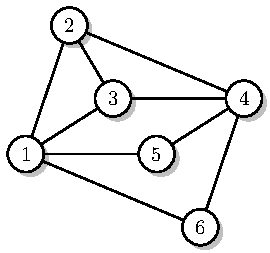
\includegraphics[width=0.35\textwidth]{Figures/FigA.pdf}
	}
	\hspace{3em} % make more space
	\subfloat[graph representation\label{fig:Subfig2}]
	{
		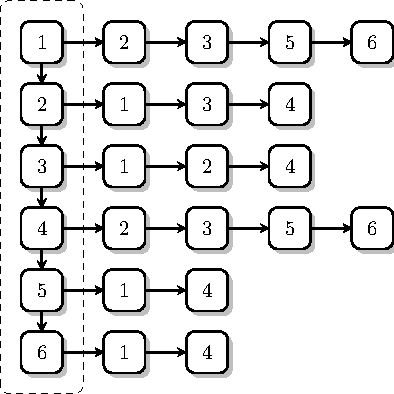
\includegraphics[width=0.35\textwidth]{Figures/FigB.pdf}
	}
	\caption{Sample figure with two subfigures}
	\label{fig:TopLevelFigureLabel}
\end{figure}

Aenean id metus id velit ullamcorper pulvinar. Excepteur sint occaecat cupidatat non proident, sunt in culpa qui officia deserunt mollit anim id est laborum. Donec quis nibh at felis congue commodo. Integer tempor. Nullam feugiat, turpis at pulvinar vulputate, erat libero tristique tellus, nec bibendum odio risus sit amet ante. Quisque tincidunt scelerisque libero. Nullam justo enim, consectetuer nec, ullamcorper ac, vestibulum in, elit. Lorem ipsum dolor sit amet, consectetuer adipiscing elit. Aliquam erat volutpat. Nullam faucibus mi quis velit. Ut enim ad minima veniam, quis nostrum exercitationem ullam corporis suscipit laboriosam, nisi ut aliquid ex ea commodi consequatur? Morbi leo mi, nonummy eget tristique non, rhoncus non leo. Maecenas lorem. Praesent id justo in neque elementum ultrices. Pellentesque sapien. In laoreet, magna id viverra tincidunt, sem odio bibendum justo, vel imperdiet sapien wisi sed libero.

Aliquam id dolor. Duis condimentum augue id magna semper rutrum. Class aptent taciti sociosqu ad litora torquent per conubia nostra, per inceptos hymenaeos. Etiam bibendum elit eget erat. Nemo enim ipsam voluptatem quia voluptas sit aspernatur aut odit aut fugit, sed quia consequuntur magni dolores eos qui ratione voluptatem sequi nesciunt. Class aptent taciti sociosqu ad litora torquent per conubia nostra, per inceptos hymenaeos. Duis viverra diam non justo. Class aptent taciti sociosqu ad litora torquent per conubia nostra, per inceptos hymenaeos. Duis ante orci, molestie vitae vehicula venenatis, tincidunt ac pede. Aliquam ornare wisi eu metus. Aenean id metus id velit ullamcorper pulvinar. Sed ut perspiciatis unde omnis iste natus error sit voluptatem accusantium doloremque laudantium, totam rem aperiam, eaque ipsa quae ab illo inventore veritatis et quasi architecto beatae vitae dicta sunt explicabo. Duis aute irure dolor in reprehenderit in voluptate velit esse cillum dolore eu fugiat nulla pariatur. Nullam rhoncus aliquam metus. Maecenas libero. Proin mattis lacinia justo. Nulla non lectus sed nisl molestie malesuada. Etiam quis quam. Ut enim ad minima veniam, quis nostrum exercitationem ullam corporis suscipit laboriosam, nisi ut aliquid ex ea commodi consequatur?

\section{Aliquam Ornare Wisi Metus}
Maecenas ipsum velit, consectetuer eu lobortis ut, dictum at dui. Duis sapien nunc, commodo et, interdum suscipit, sollicitudin et, dolor. Aliquam in lorem sit amet leo accumsan lacinia. Vivamus luctus egestas leo. Sed elit dui, pellentesque a, faucibus vel, interdum nec, diam. Nullam eget nisl. Nemo enim ipsam voluptatem quia voluptas sit aspernatur aut odit aut fugit, sed quia consequuntur magni dolores eos qui ratione voluptatem sequi nesciunt. Duis condimentum augue id magna semper rutrum. Fusce aliquam vestibulum ipsum. Lorem ipsum dolor sit amet, consectetuer adipiscing elit.

In sem justo, commodo ut, suscipit at, pharetra vitae, orci. Maecenas fermentum, sem in pharetra pellentesque, velit turpis volutpat ante, in pharetra metus odio a lectus. Aliquam erat volutpat. Sed ac dolor sit amet purus malesuada congue. Aliquam erat volutpat. Quisque porta. Temporibus autem quibusdam et aut officiis debitis aut rerum necessitatibus saepe eveniet ut et voluptates repudiandae sint et molestiae non recusandae. Nullam sapien sem, ornare ac, nonummy non, lobortis a enim. Nullam dapibus fermentum ipsum. In rutrum. Morbi scelerisque luctus velit. Donec ipsum massa, ullamcorper in, auctor et, scelerisque sed, est. Ut enim ad minim veniam, quis nostrud exercitation ullamco laboris nisi ut aliquip ex ea commodo consequat.
\endinput
\chapter{Technical Details}
\section{Cross References}
\label{sec:CrossReferences}
There are usually a lot of cross references in scientific texts or in a thesis. Typical entities referred to in the text are:
\begin{description}
	\item [sections] -- for example section \ref{sec:ExpeditaDistinctio}. If we refer to a section that is very far from the current page, it is usual to include the corresponding page number with the section number, such as section \ref{sec:Introduction} on page \pageref{sec:Introduction}.
	\item [figures] -- for example figures \ref{fig:WritingThesis}, \ref{fig:CoffeAndComputerInAppendix}, and \ref{fig:TSquareFractal}. We can also refer to high level figures, e.g.\ figure \ref{fig:TopLevelFigureLabel}, which are divided into separate subfigures such as \ref{fig:Subfig1} and \ref{fig:Subfig2}.
	\item [tables] -- for example tables \ref{tab:ExpResults} and \ref{tab:Sidewaystable}. There is high level table \ref{tab:TopLevelTableLabel} and subtables \ref{tab:Subtable1} and \ref{tab:Subtable2} too.
	\item [equations] -- equation numbers are usually enclosed by parentheses, such as equation (\ref{eq:A}), (\ref{eq:B}) or (\ref{eq:C}).
	\item [source code listings] -- for example listing \ref{src:CppListing}. The listing \ref{src:PythonListing} is an example of listing in different language, in this case Python, than the default C++. We can also refer to long listing, such as listing \ref{src:CppExternal} on page \pageref{src:CppExternal} in appendix \ref{sec:Appendix1}, which is loaded form external source code file.
\end{description}

\section{How to cite}
\label{sec:HowToCite}
\subsection{In-text citing}
It is not necessary to mention an author's name, pages used, or date of publication in the in-text citation. Instead, refer to the source with a number in a square bracket, e.g. [1], that will then correspond to the full citation in your reference list. For example we can cite resources like \emph{articles} \cite{herrmann, bertram, moore, yoon, sigfridsson, baez/article}, \emph{books} \cite{wilde, nietzsche:ksa1, averroes/bland, hammond, cotton, knuth:ct:a, gerhardt, gonzalez, companion}, \emph{periodicals} \cite{jcg}, \emph{theses} \cite{geer}, \emph{patents} \cite{kowalik, almendro, sorace, laufenberg}, \emph{online resources} \cite{ctan, wassenberg, itzhaki, markey, baez/online}, \emph{manuals} \cite{cms}.

\subsection{Creating a Reference List}
The Reference List appears at the end of your thesis and provides the full citations for all the references you have used.  

\section{How to compile}
To build this thesis demo from scratch you have to run pdf\LaTeX{} and Biber several times in following way:
\begin{verbatim}
pdflatex <main file name>
biber <main file name>
pdflatex <main file name>
pdflatex <main file name>
pdflatex <main file name>
\end{verbatim}
\endinput
\chapter{Conclusion}
Donec iaculis gravida nulla. Mauris metus. Pellentesque pretium lectus id turpis. Proin in tellus sit amet nibh dignissim sagittis. Integer pellentesque quam vel velit. Duis pulvinar. Nulla non arcu lacinia neque faucibus fringilla. Aliquam erat volutpat. Pellentesque arcu. Cras elementum. Nulla est. Fusce dui leo, imperdiet in, aliquam sit amet, feugiat eu, orci. Fusce aliquam vestibulum ipsum. Nam libero tempore, cum soluta nobis est eligendi optio cumque nihil impedit quo minus id quod maxime placeat facere possimus, omnis voluptas assumenda est, omnis dolor repellendus. Pellentesque pretium lectus id turpis.

Maecenas fermentum, sem in pharetra pellentesque, velit turpis volutpat ante, in pharetra metus odio a lectus. Nunc auctor. Fusce consectetuer risus a nunc. Curabitur sagittis hendrerit ante. Nulla non arcu lacinia neque faucibus fringilla. Cras elementum. Itaque earum rerum hic tenetur a sapiente delectus, ut aut reiciendis voluptatibus maiores alias consequatur aut perferendis doloribus asperiores repellat. In rutrum. Nullam at arcu a est sollicitudin euismod. Neque porro quisquam est, qui dolorem ipsum quia dolor sit amet, consectetur, adipisci velit, sed quia non numquam eius modi tempora incidunt ut labore et dolore magnam aliquam quaerat voluptatem. Integer in sapien.

Class aptent taciti sociosqu ad litora torquent per conubia nostra, per inceptos hymenaeos. Integer malesuada. Pellentesque arcu. Lorem ipsum dolor sit amet, consectetuer adipiscing elit. Duis viverra diam non justo. Ut tempus purus at lorem. Aliquam erat volutpat. Sed vel lectus. Donec odio tempus molestie, porttitor ut, iaculis quis, sem. Fusce wisi. Morbi leo mi, nonummy eget tristique non, rhoncus non leo. Aliquam ornare wisi eu metus. Itaque earum rerum hic tenetur a sapiente delectus, ut aut reiciendis voluptatibus maiores alias consequatur aut perferendis doloribus asperiores repellat. Aliquam ante. Quisque tincidunt scelerisque libero.

Sed elit dui, pellentesque a, faucibus vel, interdum nec, diam. Aliquam in lorem sit amet leo accumsan lacinia. Neque porro quisquam est, qui dolorem ipsum quia dolor sit amet, consectetur, adipisci velit, sed quia non numquam eius modi tempora incidunt ut labore et dolore magnam aliquam quaerat voluptatem. Mauris metus. Etiam ligula pede, sagittis quis, interdum ultricies, scelerisque eu. Fusce aliquam vestibulum ipsum. Nulla non arcu lacinia neque faucibus fringilla. Mauris suscipit, ligula sit amet pharetra semper, nibh ante cursus purus, vel sagittis velit mauris vel metus. Vestibulum erat nulla, ullamcorper nec, rutrum non, nonummy ac, erat. Mauris tincidunt sem sed arcu. Curabitur sagittis hendrerit ante. Vivamus ac leo pretium faucibus. Duis sapien nunc, commodo et, interdum suscipit, sollicitudin et, dolor.

Excepteur sint occaecat cupidatat non proident, sunt in culpa qui officia deserunt mollit anim id est laborum. Pellentesque sapien. Mauris elementum mauris vitae tortor. Vestibulum erat nulla, ullamcorper nec, rutrum non, nonummy ac, erat. Duis ante orci, molestie vitae vehicula venenatis, tincidunt ac pede. Proin pede metus, vulputate nec, fermentum fringilla, vehicula vitae, justo. Cras pede libero, dapibus nec, pretium sit amet, tempor quis. In sem justo, commodo ut, suscipit at, pharetra vitae, orci. Mauris metus. Donec ipsum massa, ullamcorper in, auctor et, scelerisque sed, est.

Etiam ligula pede, sagittis quis, interdum ultricies, scelerisque eu. In enim a arcu imperdiet malesuada. Nunc auctor. Proin mattis lacinia justo. Nemo enim ipsam voluptatem quia voluptas sit aspernatur aut odit aut fugit, sed quia consequuntur magni dolores eos qui ratione voluptatem sequi nesciunt. In rutrum. Et harum quidem rerum facilis est et expedita distinctio. Curabitur vitae diam non enim vestibulum interdum. Fusce tellus odio, dapibus id fermentum quis, suscipit id erat. Aliquam erat volutpat. Integer lacinia. Nam quis nulla. Aliquam id dolor. Nunc auctor. Aliquam erat volutpat. Aenean vel massa quis mauris vehicula lacinia.
\endinput


\printbibliography[heading=bibintoc]

\appendix
\chapter{Etiam Sapien Elit Consequat Eget}
Vestibulum fermentum tortor id mi. Etiam ligula pede, sagittis quis, interdum ultricies, scelerisque eu. Pellentesque sapien. Integer in sapien. Et harum quidem rerum facilis est et expedita distinctio. Class aptent taciti sociosqu ad litora torquent per conubia nostra, per inceptos hymenaeos. Aliquam ornare wisi eu metus. Nullam sapien sem, ornare ac, nonummy non, lobortis a enim. Etiam sapien elit, consequat eget, tristique non, venenatis quis, ante. Nullam sit amet magna in magna gravida vehicula. Sed vel lectus. Donec odio tempus molestie, porttitor ut, iaculis quis, sem. Mauris tincidunt sem sed arcu. Lorem ipsum dolor sit amet, consectetuer adipiscing elit. Duis ante orci, molestie vitae vehicula venenatis, tincidunt ac pede. Sed vel lectus. Donec odio tempus molestie, porttitor ut, iaculis quis, sem. Mauris elementum mauris vitae tortor. Nunc dapibus tortor vel mi dapibus sollicitudin. Mauris dolor felis, sagittis at, luctus sed, aliquam non, tellus. Quisque tincidunt scelerisque libero.

Aliquam ornare wisi eu metus. Etiam ligula pede, sagittis quis, interdum ultricies, scelerisque eu. Pellentesque habitant morbi tristique senectus et netus et malesuada fames ac turpis egestas. Ut tempus purus at lorem. Quisque porta. Maecenas ipsum velit, consectetuer eu lobortis ut, dictum at dui. Temporibus autem quibusdam et aut officiis debitis aut rerum necessitatibus saepe eveniet ut et voluptates repudiandae sint et molestiae non recusandae. Vivamus luctus egestas leo. Nullam justo enim, consectetuer nec, ullamcorper ac, vestibulum in, elit. Nullam dapibus fermentum ipsum. Cras pede libero, dapibus nec, pretium sit amet, tempor quis. Maecenas fermentum, sem in pharetra pellentesque, velit turpis volutpat ante, in pharetra metus odio a lectus. Nulla non lectus sed nisl molestie malesuada. Duis pulvinar. Vestibulum erat nulla, ullamcorper nec, rutrum non, nonummy ac, erat. Cras elementum. Donec quis nibh at felis congue commodo. Maecenas aliquet accumsan leo.

Etiam dui sem, fermentum vitae, sagittis id, malesuada in, quam. In laoreet, magna id viverra tincidunt, sem odio bibendum justo, vel imperdiet sapien wisi sed libero. Aliquam erat volutpat. Integer tempor. Quisque porta. Etiam egestas wisi a erat. Nulla accumsan, elit sit amet varius semper, nulla mauris mollis quam, tempor suscipit diam nulla vel leo. Duis aute irure dolor in reprehenderit in voluptate velit esse cillum dolore eu fugiat nulla pariatur. Curabitur ligula sapien, pulvinar a vestibulum quis, facilisis vel sapien. Nam quis nulla. Nemo enim ipsam voluptatem quia voluptas sit aspernatur aut odit aut fugit, sed quia consequuntur magni dolores eos qui ratione voluptatem sequi nesciunt. Fusce consectetuer risus a nunc. Etiam quis quam. Cum sociis natoque penatibus et magnis dis parturient montes, nascetur ridiculus mus. Nam sed tellus id magna elementum tincidunt. Aenean fermentum risus id tortor.

Nam libero tempore, cum soluta nobis est eligendi optio cumque nihil impedit quo minus id quod maxime placeat facere possimus, omnis voluptas assumenda est, omnis dolor repellendus. Ut enim ad minima veniam, quis nostrum exercitationem ullam corporis suscipit laboriosam, nisi ut aliquid ex ea commodi consequatur? Duis condimentum augue id magna semper rutrum. In dapibus augue non sapien. Curabitur bibendum justo non orci. Quis autem vel eum iure reprehenderit qui in ea voluptate velit esse quam nihil molestiae consequatur, vel illum qui dolorem eum fugiat quo voluptas nulla pariatur? Integer rutrum, orci vestibulum ullamcorper ultricies, lacus quam ultricies odio, vitae placerat pede sem sit amet enim. Sed elit dui, pellentesque a, faucibus vel, interdum nec, diam. Nullam justo enim, consectetuer nec, ullamcorper ac, vestibulum in, elit. In enim a arcu imperdiet malesuada. Morbi scelerisque luctus velit. Nulla quis diam. Et harum quidem rerum facilis est et expedita distinctio. Mauris elementum mauris vitae tortor. Sed vel lectus. Donec odio tempus molestie, porttitor ut, iaculis quis, sem. Aenean placerat. In sem justo, commodo ut, suscipit at, pharetra vitae, orci. Mauris tincidunt sem sed arcu.\endinput
\chapter{Large Figures and Tables}
\label{sec:Appendix1}
\begin{figure}[!h]
	\centering
	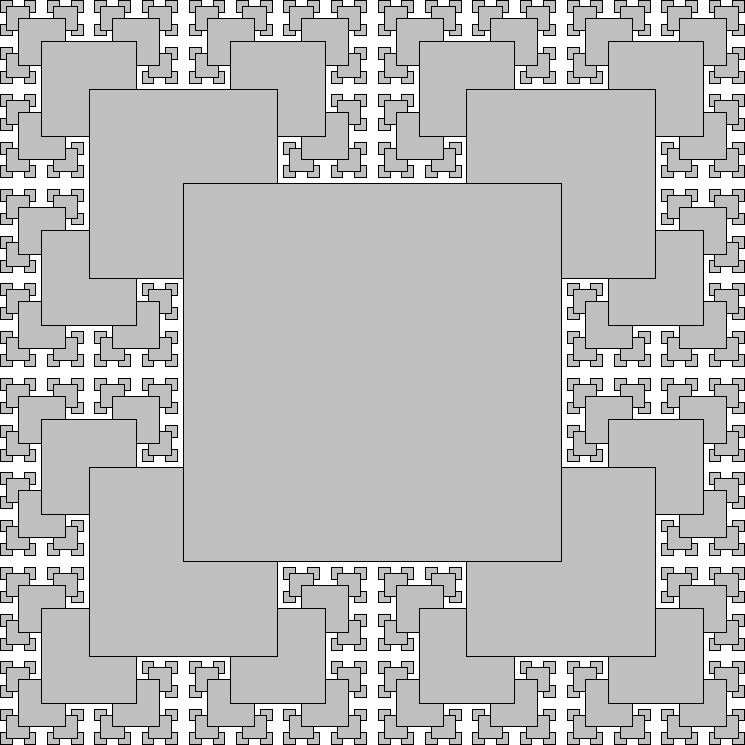
\includegraphics[width=0.8\textwidth]{Figures/FigC.pdf}
	\caption{T-square fractal}
	\label{fig:TSquareFractal}
\end{figure}


\begin{sidewaystable}
	\centering
	\caption{Large table example with columns aligned in different ways}
	\label{tab:Sidewaystable}
\begin{tabular}{rrrlcp{95mm}}
\toprule
Right	&	Right	&	Right	&	Left					&	Center	&	Paragraph	\\
\midrule
-7576	&	-2092	&	5418	&	nulla pulvinar			&	a		&	Donec ipsum massa, ullamcorper in, auctor et, scelerisque sed.	\\
-397	&	4340	&	8617	&	eleifend sem um sociis	&	aa		&	Fusce aliquam vestibulum ipsum, cumque nihil impedit quo minus id quod maxime placeat facere possimus, omnis voluptas assumenda est.	\\
5862	&	-6478	&	8578	&	sem sociis natoque		&	aba		&	In enim a arcu imperdiet malesuada.	\\
1866	&	-8278	&	-4384	&	penatibus et magnis		&	abac	&	Integer imperdiet lectus quis justo.	\\
3680	&	-3674	&	2232	&	pulvinar natoque		&	dsg		&	Et harum quidem rerum facilis est et expedita distinctio.	\\
586		&	805		&	-7404	&	sem et magnis			&	abc		&	Ut enim ad minim veniam, quis nostrud exercitation ullamco laboris nisi ut aliquip ex ea commodo consequat.	\\
1388	&	8761	&	-8929	&	sem odio bibendum		&	tsi		&	Phasellus faucibus molestie nisl.	\\
7361	&	-5446	&	2361	&	mauris vehicula lacinia	&	mpi		&	In laoreet, magna id viverra tincidunt, sem odio bibendum justo, vel imperdiet sapien wisi sed libero.	\\
-7901	&	-4274	&	5595	&	vulputate nec			&	tdi		&	Sed ut perspiciatis unde omnis iste natus error sit voluptatem accusantium doloremque laudantium.	\\
-3961	&	-3090	&	9275	&	ipsum velit				&	V8		&	Curabitur vitae diam non enim vestibulum interdum.	\\
\bottomrule
\end{tabular}
\end{sidewaystable}


\begin{sidewaysfigure}
	\centering
	
\includegraphics[width=0.95\textwidth]{Figures/CoffeeAndComputer.jpg}
	\caption{Coffee and computer \cite{AhDTEmY2CY7Qv65e}}
	\label{fig:CoffeAndComputerInAppendix}
\end{sidewaysfigure}
\endinput


% Appendix included directly in main LaTeX file. Not all attachments need to be in separate files.
\chapter{Long Source Code Listing}
\lstinputlisting[label=src:CppExternal,caption={Long C++ source code taken from external file}]{SourceCodes/ArraySortingAlgorithms.cpp}

\end{document}
